\documentclass[twocolumn]{iopjournal}

\usepackage{amsmath,amssymb,amsfonts}
\usepackage{tikz}

\fancyhfoffset[L]{0mm}
\setlength{\marginparwidth}{0pt}
\setlength{\marginparsep}{0pt}

% ==========================================
% ZENODO PREPRINT HEADERS (ACTIVE)
% ==========================================
\renewcommand{\articletype}[1]{%
  {\vspace*{-8mm}\noindent \Large \sf Preprint}\par
  \vspace*{6mm}\noindent{\scriptsize \sf{\bfseries \MakeUppercase{#1}}}}

\fancyhead[L]{}
\fancyhead[R]{}

% ==========================================
% CQG SUBMISSION HEADERS (COMMENTED OUT)
% ==========================================
% \fancyhead[L]{{\small \sf IOP Publishing}\hspace{5mm} {\it Class. Quantum Grav.}}
% \fancyhead[R]{S Nelson}

\begin{document}

\articletype{Letter}

\title{The Coordinate-Space Geometry of the Tetrad Frame}

\author{Stephen Nelson}

\affil{Field Dynamics Research}

\ead{stephen@fielddynamics.org}

\begin{abstract}
The tetrad (vierbein) is the local orthonormal frame on which the coupling of gravity to fermionic matter depends, yet its coordinate-space geometry has not, to our knowledge, been examined. Deriving four oriented half-space inequalities from the spatial sector of a single orthonormal tetrad, the $2^4 = 16$ possible sign combinations yield exactly two bounded regions. The bounded pair form a stellated octahedron whose boundary decomposes into sixteen independent channels. No dual frame is introduced; the orientation-reversed tetrahedral sector emerges as the unique second bounded region of the same single-tetrad construction. All structural constants of the resulting geometry reduce to two integers: the number of tetrahedral faces $K = 4$ and the spatial dimension $D = 3$. A numerical rendering at four million sample points confirms the derived structure.
\end{abstract}

% ----------------------------------------------------------------------

\section*{Introduction}

General relativity is most commonly formulated in terms of the metric tensor $g_{\mu\nu}$, a symmetric matrix encoding distances and angles in curved spacetime. There is, however, a deeper formulation. The \emph{tetrad} (or \emph{vierbein}) $e^a{}_\mu$ is a set of four vector fields that serve as a local orthonormal frame at each point of the manifold. The metric is recovered as a derived quantity,
\begin{equation}
g_{\mu\nu} = \eta_{ab}\, e^a{}_\mu\, e^b{}_\nu,
\end{equation}
making the tetrad, in a precise algebraic sense, the square root of the metric. The flat metric $\eta_{ab}$ in this expression carries the Lorentz signature $(-,+,+,+)$, one timelike dimension and three spacelike dimensions, and so the tetrad's four legs reflect this $3+1$ decomposition directly, one spanning the local time direction and three spanning the local spatial frame.

Coupling fermions (electrons, quarks, neutrinos) to gravity requires the local Lorentz frame that only the tetrad provides, making this formulation not an alternative to general relativity but its most fundamental expression. The approach has been standard since the work of Cartan, Einstein~\cite{Einstein1928}, and Weyl~\cite{Weyl1929}, and underpins modern frameworks including Poincar\'{e} gauge gravity~\cite{Hehl1976}, Ashtekar variables~\cite{Ashtekar1986}, loop quantum gravity, bimetric gravity~\cite{HassanRosen2012}, and supergravity.

Despite this centrality, the tetrad formalism is almost always presented in index notation: $e^a{}_\mu$ carrying a Lorentz index $a$ and a spacetime index $\mu$. The indices are manipulated algebraically, but in over a century of use, the spatial structure that these four vector fields generate has not, to our knowledge, been rendered in coordinate space.

This paper does that. We write the tetrad's spatial components as explicit half-space inequalities and derive the geometry that their half-space combinations produce; a numerical rendering confirms the result visually, but the argument is analytic.

We do not begin with a stellated octahedron, nor with a pair of dual tetrahedra. We begin with a single orthonormal tetrad. The opposite-oriented tetrahedral sector appears as a necessary consequence of the half-space structure that the tetrad's four planes generate.

\begin{figure}[t]
\centering
\includegraphics[width=\columnwidth]{fig1_tetrad_frame}
\caption{The coordinate-space geometry of the tetrad frame. Four million points are sampled uniformly in local frame coordinates and classified by the sign combination each point occupies under the four projections $v_i$. The primary tetrahedron (TetA) appears in blue, a second inverted tetrahedron (TetB) in red, and their shared interior, a regular octahedron, in gold. The geometry is analysed in the text. An interactive HTML rendering is provided as supplementary material.}
\label{fig1}
\end{figure}

% ----------------------------------------------------------------------

\section*{Four Planes}

The $(-,+,+,+)$ signature maps null directions in the local frame to
the unit sphere $S^2$. The three identical spacelike entries give the
spatial sector full $SO(3)$ invariance; requiring that a discrete
four-direction set on $S^2$ introduce no net preferred spatial direction
uniquely fixes the regular tetrahedral frame with pairwise inner product
$c = -1/3$ (proved in Supplementary Material, Proposition). The four directions,
expressed as linear projections of the local coordinates, are:
\begin{align}
v_1 &= x + y + z, \nonumber \\
v_2 &= x - y - z, \nonumber \\
v_3 &= -x + y - z, \nonumber \\
v_4 &= -x - y + z.
\end{align}

Each projection $v_i$ defines a half-space: the set of all points on one side of the corresponding plane $v_i = \mathrm{const}$. The four planes together close to form a tetrahedron, the unique bounded solid that four planes can enclose. The region where all four projections are simultaneously bounded defines the primary tetrahedral frame, which we label TetA:
\begin{equation}
\textbf{TetA}: \quad \max(v_1,\, v_2,\, v_3,\, v_4) \leq 1.
\end{equation}

Each $v_i$ is the dot product of the position vector with one of the four directions derived above; it measures the displacement of a point along that direction. These projections encode the tetrad's spatial sector in its unique isotropic four-direction basis, playing the role of spatial one-forms projected along the tetrahedral normals rather than the three orthogonal legs. Bounding them as half-space inequalities makes the tetrad's spatial geometry directly computable.

To render this geometry, we sample four million points uniformly in a cube of local frame coordinates, evaluate the four inequalities at each point, and colour each point according to the region it occupies. The geometry emerges from the half-space boundaries alone, without mesh construction or surface fitting. Figure~\ref{fig1} confirms the analytically derived structure described in the following section.

% ----------------------------------------------------------------------

\section*{The Emergent Geometry}

Figure~\ref{fig1} displays the geometry that the four half-space
inequalities produce. The rendering reveals two tetrahedral regions, one
upright (blue) and one inverted (red), overlapping around a compact gold
core. All three regions emerge from the same four planes defined in the
previous section. This section proves which regions must close into finite
solids, why no others can, and identifies the composite solid they form.

Each projection $v_i$ divides coordinate space with a bounding plane. On
one side lies the half-space $\{v_i \leq 1\}$; on the other, its
complement. Replacing $v_i$ with $-v_i$ and applying the same bound gives
the opposite half-space $\{-v_i \leq 1\}$. Since there are four
projections, each offering two choices, there are $2^4 = 16$ ways to
select one half-space per projection. Each selection produces a convex
region, the intersection of four half-spaces. A bounded intersection
closes on itself to form a finite solid; an unbounded one extends to
infinity and has no geometric identity. The natural question is: which of
these sixteen regions are bounded? The answer turns on a single algebraic
identity among the four projections.

In three spatial dimensions, four unit vectors with equal pairwise angles
admit no other configuration than the face normals of a regular
tetrahedron, and face normals of a regular tetrahedron sum to zero. The
four projections therefore satisfy
\begin{equation}
v_1 + v_2 + v_3 + v_4 = 0.
\end{equation}
This identity holds at every point in coordinate space and is the sole
algebraic relation among the four projections. When the inward-pointing
normals of a set of bounding planes sum to zero, the origin sits at their
centroid, strictly inside their convex hull, and the walls close from
every direction; when they do not, a gap opens and the region escapes to
infinity. For TetA, the four inward normals are the derived tetrahedral
directions; they sum to zero, so TetA is bounded. This is unsurprising;
TetA was defined by bounding all four projections.

But the same argument applies to the four negated directions: they also sum to
zero, placing the origin at their centroid. A second bounded region
exists, one that was never defined or constructed. This is TetB:
\begin{equation}
\textbf{TetB}: \quad \max(-v_1,\, -v_2,\, -v_3,\, -v_4) \leq 1.
\end{equation}

No other region can be bounded. Consider any mixed selection, say three
directions that keep their original orientation and one that is flipped. The
linear relation means the flipped direction equals the sum of the other three:
it is a positive combination of them. All four selected normals therefore
point into the same half of space, the origin lies outside their convex
hull, and the region escapes to infinity. The same reasoning applies to
every other mixed selection: flipping any strict subset of the directions breaks
the surrounding property, and the intersection is unbounded. Of the
sixteen regions, exactly two close into finite solids: in
Figure~\ref{fig1}, the blue region is TetA and the red region is TetB.
The orientation-reversed tetrahedral sector was not introduced as a
separate frame; it emerges as the unique second bounded region among the
sixteen half-space combinations of a single orthonormal tetrad.

The two tetrahedra interpenetrate: each vertex of TetB passes through a
face of TetA, and each vertex of TetA passes through a face of TetB.
Their intersection is the set of points satisfying $|v_i| \leq 1$ for all
$i$. This region has six vertices, each obtained by setting one
$|v_i| = 1$ and solving for the remaining three under the constraint
$\sum v_i = 0$; all twelve edges are equal in length. The intersection is
therefore a regular octahedron, visible as the gold core at the centre of
Figure~\ref{fig1}. The union of the two tetrahedra is a stellated
octahedron, first described by Kepler~\cite{Kepler1619} and known in
modern polyhedral geometry as the stella
octangula~\cite{Cromwell1997}, here derived from the half-space inequalities
of a single orthonormal tetrad.

This interpenetration couples all four faces of each tetrahedron. On each
of the four coupled faces, the opposing vertex carves the face into four
distinct sub-regions: three exposed triangular corners and one central
inverted core. The resulting pattern is the
first level of a Sierpinski subdivision, visible on every face in
Figure~\ref{fig1}. The total number of independent boundary channels
across the four coupled faces follows immediately:
\begin{equation}
4 \;\text{faces} \times 4 \;\text{sub-regions} = 16 \;\text{channels}.
\label{eq:channels}
\end{equation}
Each channel is a distinct connected region of the boundary surface,
separated from its neighbours by the edges where TetA and TetB intersect.
Figure~\ref{fig2} illustrates the subdivision for a single face; the
numerical rendering at four million sample points confirms the full count.
Whether deeper levels of the Sierpinski recursion carry geometric
significance is not addressed here.

\begin{figure}[t]
\centering
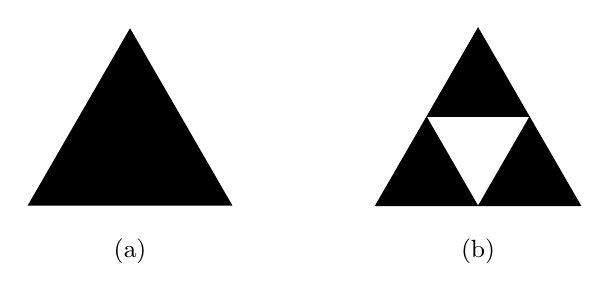
\begin{tikzpicture}[scale=1.3]
  % Panel (a): one solid face of TetA
  \fill[black] (0,0) -- (2,0) -- (1,1.732) -- cycle;
  \node at (1,-0.45) {\small (a)};

  % Panel (b): the same face after TetB's vertex penetrates
  \begin{scope}[xshift=3.4cm]
    \fill[black] (0,0) -- (1,0) -- (0.5,0.866) -- cycle;
    \fill[black] (1,0) -- (2,0) -- (1.5,0.866) -- cycle;
    \fill[black] (0.5,0.866) -- (1.5,0.866) -- (1,1.732) -- cycle;
    \draw[black, line width=0.4pt] (0,0) -- (2,0) -- (1,1.732) -- cycle;
    \node at (1,-0.45) {\small (b)};
  \end{scope}
\end{tikzpicture}
\caption{The face subdivision. (a)~One face of TetA, undivided. (b)~The opposing vertex of TetB penetrates the face, carving it into three exposed corners and one central inverted core. This $3+1$ pattern is the first Sierpinski iteration and repeats on all four faces, producing the $4 \times 4 = 16$ boundary channels of Eq.~(\ref{eq:channels}).}
\label{fig2}
\end{figure}

The three regions visible in Figure~\ref{fig1} are now fully accounted
for. The blue and red tetrahedra are the only bounded regions among the
sixteen half-space combinations; the gold octahedron is their intersection;
and the composite stellated octahedron, with its sixteen boundary channels,
is generated by the half-space inequalities of a single orthonormal tetrad,
with nothing introduced and nothing added.

% ----------------------------------------------------------------------

\section*{Structural Inventory}

Every structural constant of the stellated octahedron that the tetrad produces reduces to two integers: the number of faces per tetrahedron, $K = 4$, and the spatial dimension, $D = 3$. In combinatorial topology, the standard inventory of a polyhedron is its f-vector $(f_0, f_1, f_2)$, recording the number of vertices, edges, and faces. This count is a coordinate-independent combinatorial inventory.

\vspace{6pt}
\noindent
\begin{tabular*}{\columnwidth}{@{\extracolsep{\fill}}lcc@{}}
\hline
Quantity & Expression & Value \\
\hline
Tetrahedra (TetA, TetB) & $2$ & 2 \\
Faces per tetrahedron & $K$ & 4 \\
Vertices (total) & $2^D$ & 8 \\
Edges (total) & $K \times D$ & 12 \\
Faces (total) & $2K$ & 8 \\
Boundary channels & $K^2$ & 16 \\
f-vector sum ($V\!+\!E\!+\!F$) & $K(K\!+\!D)$ & 28 \\
\hline
\end{tabular*}
\vspace{6pt}

\noindent
The f-vector of the stellated octahedron is $(8, 12, 8)$, giving a total element count of $V + E + F = 28$. The alternating sum $V - E + F = 4$ equals twice the Euler characteristic of a sphere, consistent with two simplicially disjoint closed surfaces. Every entry in the table is determined by $K$ and $D$ alone. No additional parameters or geometric inputs are required.

% ----------------------------------------------------------------------

\section*{Discussion}

The preceding sections derived both tetrahedra, their interpenetration, and all sixteen boundary channels from a single input: the four half-space inequalities of one orthonormal tetrad. Of the sixteen sign combinations, exactly two are bounded, and the dual frame emerges as an analytic consequence of the primary frame's four planes. Each tetrahedron individually carries a $3+1$ face decomposition: one face whose normal has uniform sign and three faces with mixed signs, mirroring the $(-,+,+,+)$ Lorentz signature from which the construction began.

The introduction noted that the tetrad is, algebraically, the square root of the metric. Because the metric depends quadratically on the tetrad, parity-related spatial frame realisations produce the same $g_{\mu\nu}$. The two bounded regions derived above are the coordinate-space realisation of that doubled frame structure: TetA and TetB are distinct tetrad-level realisations of the same metric.

The geometry reported here is not contingent on a particular gravitational action or field equation. The two interpenetrating tetrahedra, the octahedral intersection, and the sixteen boundary channels are consequences of the tetrad's combinatorial structure (four derived directions in three spatial dimensions) and are present before any dynamics are imposed. This geometry is consequently present in the local frame of any covariant theory formulated in the tetrad variables.

% ----------------------------------------------------------------------

\section*{Data and Reproducibility}

The point-cloud visualisation in Figure~\ref{fig1} was generated by
evaluating the four tetrahedral half-space inequalities at four million
uniformly sampled points. The rendering code is provided as an interactive
HTML file (\texttt{fig1\_tetrad\_frame.html}) included
as supplementary material. A self-contained validation script
(\texttt{run\_all\_validations.py}) independently verifies every geometric
claim in this paper, requiring only NumPy and SciPy. A derivation of the
tetrahedral frame from the Lorentz signature is provided as a separate
supplementary note (\texttt{supplementary\_signature\_to\_frame.pdf}).
An independent derivation of the two bounded regions from the quadratic
structure of the tetrad equation is provided as a second supplementary
note (\texttt{supplementary\_scheme\_proof.pdf}).

% ----------------------------------------------------------------------

\begin{thebibliography}{99}

\bibitem{Einstein1928}
A.~Einstein,
``Riemann-Geometrie mit Aufrechterhaltung des Begriffes des Fernparallelismus,''
\textit{Sitzungsber. Preuss. Akad. Wiss.} (1928), 217.

\bibitem{Weyl1929}
H.~Weyl,
``Elektron und Gravitation. I,''
\textit{Z. Phys.} \textbf{56}, 330 (1929).

\bibitem{Hehl1976}
F.~W.~Hehl, P.~von~der~Heyde, G.~D.~Kerlick and J.~M.~Nester,
``General relativity with spin and torsion: Foundations and prospects,''
\textit{Rev. Mod. Phys.} \textbf{48}, 393 (1976).

\bibitem{Ashtekar1986}
A.~Ashtekar,
``New variables for classical and quantum gravity,''
\textit{Phys. Rev. Lett.} \textbf{57}, 2244 (1986).

\bibitem{HassanRosen2012}
S.~F.~Hassan and R.~A.~Rosen,
``Bimetric gravity from ghost-free massive gravity,''
\textit{J. High Energy Phys.} \textbf{2012}(02), 126 (2012).

\bibitem{Kepler1619}
J.~Kepler,
\textit{Harmonices Mundi} (1619).

\bibitem{Cromwell1997}
P.~R.~Cromwell,
\textit{Polyhedra}
(Cambridge University Press, Cambridge, 1997).

\end{thebibliography}

\end{document}
